\documentclass{ujs}
\usepackage[utf8x]{inputenc}
\usepackage{graphicx} %插入图片的宏包
\usepackage{float} %设置图片浮动位置的宏包
\usepackage{subfigure} %插入多图时用子图显示的宏包
\usepackage{verbatim}% 多行注释
\usepackage[framemethod=TikZ]{mdframed}
\usepackage[colorlinks,linkcolor=black]{hyperref}
\usepackage{multirow}
\usepackage{booktabs}
\usepackage{bigstrut}
\usepackage{hyperref}                      
\graphicspath{{imgs/}}
\major{CV}
\name{陆佳欢}
\stuid{3190105095}
\college{数科院}
\date{\zhtoday}
\expname{MNIST}
\major{应用数学系}
\course{基于手写数据集的CV探讨}
\begin{document}
\makecover

\fancyfoot{ }
\begin{abstract}
    本文通过在MNist数据集上通过分析各种网络结构正确认识CV,具体认识与实现模型以求更加深刻的认识计算机视觉。\par
    实验的第一部分:自制了beamer主题,目的用于报告的展示。以求达到能够清晰表达的作用,为了能够提高实验的效率,本文使用Anaconda也重新安装了pytorch\_gpu版.\par
    实验的第二部分:从五部分来建模。首先通过写MLP模型,具体且清晰的实现了一般DNN建模的步骤,并且在初步微调模型得到了test集上\textbf{97\%}的成绩。接着加大网络的深度,通过建立LeNet、AlexNet丰富了报告的内容,同时得到了更高的acc,其中LeNet跑10$epoch$模型平均准确率有\textbf{97.6\%},而AlexNet更深达到了\textbf{99.26\%},也是这5个网络中最高的acc。并且在AlexNet中,分别对比了手写以及模块化的不同,同时发现优化器在选择adam的时候再第一个epoch会出现很大的误差,而且这种情况不可逆,因而得选择SGD。接着使用GoogLeNet去加大网络的深度,使用了Inception V1块,但是遗憾的是GooLeNet在跑test的时候并未得到预期的结果。在换成SGD的情况下依旧失效,未知其原因。最后,为了避免ResNet出现同样的情况。我使用目前正在使用的fastai,使用它的轮子进行\textbf{迁移学习}。分别跑了ResNet18以及ResNet34得到acc分别是99\%、98\%。模型的网络变深,test的结果反倒变差了,尽管ResNet有BN层,但是有理由相信,模型已经出现了轻微的过拟合。\par 
    实验的第三部分:在具体认识模型的同时,提供了一些提高模型准确率的数据增强手段。
    
    
\end{abstract}

\textbf{关键词:} pytorch \quad MNIST\quad GoogNet\quad ResNet\quad fastai \quad 迁移学习
\newpage
\fancyfoot[C]{\bfseries\thepage}

\thispagestyle{empty}

\tableofcontents
\newpage 

% 目录后开始计数页码
\setcounter{page}{1}

\section{安装环境}
\subsection{beamer主题的制作}
在31日下午,我考虑用PPT来介绍我实验的主题,因为这样会让我的报告做的比较有条理感,于是我考虑用beamer来展示论文的结构。主要的原因是它能节省大量的时间。于是我开始寻找本校的beamer主题。遗憾的是并没有同仁做这件事。于是,兴致使然做了beamer江苏大学的非官方版。模板的制作参考了兰州大学和东南大学以及华东师范大学的制作;其中UI部分是艺术学院一位不愿留名的女生做的。最终在31晚上做完了这个主题,并且上传了\href{https://www.latexstudio.net/}{latex}搜索江苏大学便能寻到。或者打开我的\href{https://github.com/Luhuanz/pytorch}{github} 库也能找到本次实验的全部内容。
\begin{figure}[!h]
	\centering
	
\includegraphics[width=.7\textwidth]{beamer.png}
	\caption{beamer主题图}
	\label{fig:circuitm1}
\end{figure} \par
\subsection{pytorch环境的配置}
由于我长时间使用colab以及kaggle或者云平台,我的pytorch\_gpu失效了。所以不得不考虑重新安装。
\subsubsection{Anaconda创建虚拟环境}
	\begin{enumerate}
	\item [1、]  打开\textbf{cmd}.
	\item [2、]  \textbf{conda init} 初始化.
	\item[3、]  \textbf{conda create -n pytorch python=3.7} 创建一个3.7的环境.
	\item[4、 ] \textbf{conda env list} 查看环境.
	\item[5、]  \textbf{conda  activate pytorch} 转到pyotrch虚拟环境.
	\item [6、]  pip list 查看包.
	
\end{enumerate}

\subsubsection{安装pytorch\_gpu}
	\begin{enumerate}
	\item [1、]  命令行中\textbf{nvidia-smi} 查看显卡型号.\par
	\begin{figure}[!h]
		\centering
		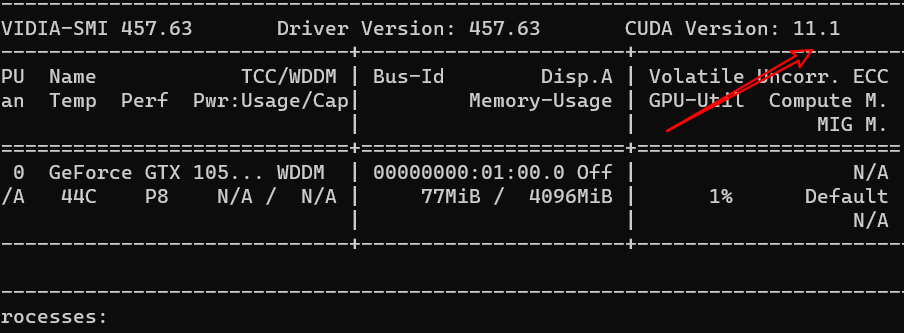
\includegraphics[width=.7\textwidth]{显卡.png}
		\caption{显卡型号11.1}
		\label{fig:circuitm1}
	\end{figure} \par
	
	\item [2、] 打开\href{https://pytorch.org/get-started/previous-versions/}{pyotch}找对应版本.
	\item[3、]  复制对应链接到cmd里注意不要直接运行. 
	\begin{figure}[!h]
		\centering
		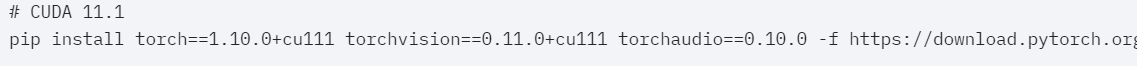
\includegraphics[width=1\textwidth]{1.png}
		\caption{我选择的版本}
		\label{fig:circuitm1}
	\end{figure} \par
	\item[4、 ]   我们需要分别安装这三个程序包,而不是网上的直接enter(会失败).
	\begin{figure}[!h]
		\centering
		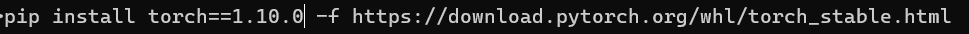
\includegraphics[width=1\textwidth]{2.png}
		\caption{演示1}
		\label{fig:circuitm1}
	\end{figure} \par 
	\begin{figure}[!h]
	\centering
	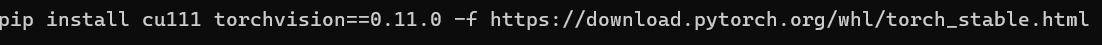
\includegraphics[width=1\textwidth]{3.png}
	\caption{演示2}
	\label{fig:circuitm1}
\end{figure} \par
	\item[5、]  接着安装\href{https://blog.csdn.net/sinat_23619409/article/details/84202651}{cuda与cudnn}	
\end{enumerate}
\begin{note}
	红色可以直接访问
\end{note}
\section{实验部分}
\subsection{MLP}
 MLP是多层感知机模型,也是最基本的DNN之一,本次对MNist手写数据集的MLP部分采用3层结构,分别是输入层,隐藏层,以及输出层。\\
 \begin{lstlisting}[language=python]
  flag = torch.cuda.is_available() #是否可用返回 boolean
  if flag:
  print("CUDA可使用")
  else:
  print("CUDA不可用")
  ngpu= 1 #有几张卡
  # Decide which device we want to run on
  device = torch.device("cuda:0" if (torch.cuda.is_available() and ngpu > 0) else "cpu")
  print("驱动为:",device)
  print("GPU型号: ",torch.cuda.get_device_name(0))
 \end{lstlisting}
上述代码能够输出GPU版本并且通用全部网络。\\
	\begin{figure}[!h]
	\centering
	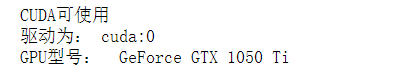
\includegraphics[width=.5\textwidth]{4.png}
	\caption{GPU}
	\label{fig:circuitm1}
\end{figure} \par
\subsubsection{MLP网络结构}
	\begin{figure}[!h]
	\centering
	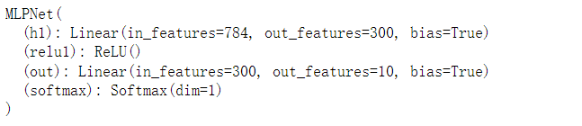
\includegraphics[width=1\textwidth]{5.png}
	\caption{MLP网络结构}
	\label{fig:circuitm1}
\end{figure} \par 
\textbf{解释说明:}输入784的神经元,然后隐层的输出为300最后输出层为10。
相当于第一层有784个节点,然后隐藏层有300个,原因在于有些没连类似Dropout,最后由于做的是10用softmax分类,所有输出层为10个节点。
\newpage
\subsubsection{train可泛化}
 \begin{lstlisting}[language=python]
	for epoch in range(num_epochs):
	for i, (x_images, y_labels) in enumerate(train_loader):
	# 因为全连接会把一行数据当做一条数据,因此我们需要将一张图片转换到一行上
	# 原始数据集的大小: [ 100, 1,28, 28]
	# resize 后的向量大小: [-1, 784]
	images = x_images.reshape(-1, 28*28).to(device)
	labels = y_labels.to(device)
	# 正向传播以及损失
	y_pre = model(images) #前向传播
	loss = criterion(y_pre, labels)# 计算损失函数
	# 反向传播
	# 梯度清空,反向传播,权重更新
	optimizer.zero_grad()#梯度归零 因为训练的过程通常使用mini-batch方法,所以如果不将梯度清零的话,梯度会与上一个batch的数据相关,因此该函数要写在反向传播和梯度下降之前。
	loss.backward()
	optimizer.step()#执行一次优化步骤,通过梯度下降法来更新参数的值。因为梯度下降是基于梯度的所以在执行optimizer.step()函数前应先执行loss.backward()函数来计算梯度。
	
	if (i+1) % 64 == 0:
	print( f'epoch [{epoch+1}/{num_epochs}], step [{i+1}/{n_total_steps}], Loss: {loss.item():.4f}')
	print("模型训练完成")
\end{lstlisting}
\subsubsection{test可泛化}
 \begin{lstlisting}[language=python]
  with torch.no_grad():
  	n_correct = 0
  	n_samples = 0
  for images, labels in test_loader:
  	images = images.reshape(-1, 28*28).to(device)
  	labels = labels.to(device)
  	outputs = model(images) 
  	_, predicted = torch.max(outputs.data, 1)
  	n_samples += labels.size(0)
  	n_correct += (predicted == labels).sum().item()
  	acc = 100.0 * n_correct / n_samples
  print(f'Accuracy of the network on the 10000 test images: {acc} %')
  
\end{lstlisting}
\subsubsection{准确率}

	\begin{figure}[!h]
	\centering
	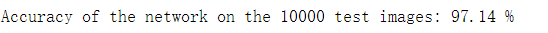
\includegraphics[width=.7\textwidth]{6.png}
	\caption{MLP网络准确率}
	\label{fig:circuitm1}
\end{figure} \par
\subsection{LeNet}
LeNet-5网络的默认的输入图片的尺寸是32*32, 而Mnist数据集的图片的尺寸是28 * 28,
因此,采用Mnist数据集时,每一层的输出的特征值feature map的尺寸与LeNet-5网络的默认默认的feature map的尺寸是不一样的,需要适当的调整。
\begin{lstlisting}[language=python]
 class LeNet(nn.Module):
 # 定义构造方法函数,用来实例化
 def __init__(self):
	 super(LeNet, self).__init__()  # 5层, 2个卷积层+3个fc全连接层
 #1*1*28*28
 # 第一个卷积层:输入通道数=1,输出通道数=6,卷积核大小=5*5,默认步长=1
	 self.conv1 = nn.Conv2d(in_channels = 1, out_channels = 6,  kernel_size = 5)   # 6 * 24 * 24 
 # 第二个卷积层:输入通道数=6,输出通道数=16,卷积核大小=5*5,默认步长=1
 	self.conv2 = nn.Conv2d(in_channels = 6, out_channels = 16, kernel_size = 5)   # 16 * 8 * 8
 
 # an affine operation: y = Wx + b
 	self.fc1 = nn.Linear(in_features = 16 * 4 * 4, out_features= 120)             # 16 * 4 * 4
	 self.fc2 = nn.Linear(in_features = 120, out_features = 84)
	 self.fc3 = nn.Linear(in_features = 84,  out_features = 10)
 # 第一个全连接层:输入特征数=256,输出特征数=120
 # 也可以理解成:将256个节点连接到120个节点上
 # 第三个全连接层:输入特征数=84,输出特征数=10(这10个维度我们作为0-9的标识来确定识别出的是那个数字。)
 # 也可以理解成:将84个节点连接到10个节点上
 def forward(self, x):
 # Max pooling over a (2, 2) window
 	x = F.max_pool2d(F.relu(self.conv1(x)),(2, 2))
	x = F.max_pool2d(F.relu(self.conv2(x)), 2)
 	x = torch.flatten(x, 1) # flatten all dimensions except the batch dimension
	x = F.relu(self.fc1(x))
 	x = F.relu(self.fc2(x))
 	x = self.fc3(x)
 #x = F.log_softmax(x,dim=1) # 这个问题前面FC建模已经说过了 参考官方LeNet
 return x
\end{lstlisting}

\begin{lstlisting}
		 输出公式 =(M-K+2P)/S +1
			M:输入神经元个数/大小
			K:卷积大小
			P:零填充
			S:步长
--------------------------------------
 第一个卷积层:self.conv1=nn.Conv2d(1,6,5) :
 其参数意义为:
     输入通道为 1 (输入图像是灰度图)
     输出通道为 6
     卷积核 kernel_size为 5×5
     24输出维度 = 28输入维度 - 5卷积核size + 1
     所以输出 shape 为:6× 24 × 24
 -----------------------------------------------------
 第一个激活函数:out = F.relu(out)
 输出维度不变仍为 6 × 24 × 24
 -----------------------------------------------------
 第一个最大池化层:out = F.max_pool2d(out, 2, 2)
     该最大池化层在 2x2 空间里向下采样。
     12输出维度 = 24输入维度 / 2。
     所以输出 shape 为:6 × 12 × 12
 -----------------------------------------------------
 第二个卷积层self.conv2=nn.Conv2d(6,16,5)
 其参数意义为:
     输入通道为 6 (第一个最大池化层的输出通道数)
     输出通道为 16 (需要用到的卷积核就有 16 种)
     卷积核kernel_size为 5×5
     8输出维度 = 12输入维度 - 5卷积核size + 1
     所以输出 shape 为:16 × 8 × 8
 ----------------------------------------------------
 第二个激活函数out = F.relu(out)
 特征提取结束
 第二个最大池化层:out = F.max_pool2d(out, 2, 2)
     该最大池化层在 2x2 空间里向下采样。
     4输出维度 = 8输入维度 / 2。
     所以输出 shape 为:16 × 4 × 4
 输出前的数据预处理
 因为全连接层Linear的输出为最后的输出,
 而全连接层Linear要求的输入为展平后的多维的卷积成的特征图(特征图为特征提取部分的结果)

 输出前的数据预处理结束
 -----------------------------------------------------
 输出即全连接层

 第一个全连接层self.fc1=nn.Linear(16*4*4, 120)
 输入维度为 16* 4 * 4= 256
 设定的输出维度为 120 × 1
 -----------------------------------------------------
 激活函数out = F.relu(out)
 输出维度不变,仍为 120 × 1
 -----------------------------------------------------
 第二个全连接层self.fc2=nn.Linear(120, 84)
 输入维度为 84
 设定的输出维度为 84 × 1
 -----------------------------------------------------
 第三个激活函数out = F.relu(x)
 输出维度不变,仍为 84× 1
 第三个全连接层self.fc3=nn.Linear(84, 10)
 输入维度为 10 × 1
 输出维度设定为 10× 1(因为是一个10分类的问题,所以最后要变成 10 × 1)
 -----------------------------------------------------
 第三个激活函数out = F.log_softmax(out, dim=1)
 用F.log_softmax()将数据的范围改到[0, 1]之内,表示概率。
 输出维度仍为 10 × 1,其值可以视为概率。
\end{lstlisting}
\subsubsection{LeNet实验结果}

\begin{figure}[!h]
	\centering
	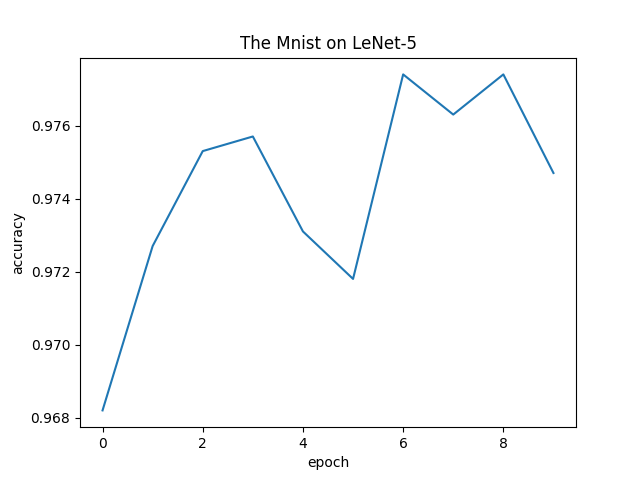
\includegraphics[width=.5\textwidth]{myplot.png}
	\caption{LeNet10\_epoch\_acc}
	\label{fig:circuitm1}
\end{figure} \par
 \noindent \textbf{10 epoch平均acc}\par
\begin{figure}[!h]
	\centering
	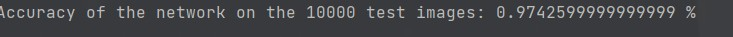
\includegraphics[width=1\textwidth]{7.jpg}
	\caption{LeNet10\_sqr\_acc}
	\label{fig:circuitm1}
\end{figure} \par
\subsection{AlexNet}
\subsubsection{AlexNet手写}
 \begin{lstlisting}[language=python]
 class AlexNet(nn.Module):
 # 定义构造方法函数,用来实例化
 	def __init__(self):
 		super(AlexNet, self).__init__()  #  
 		self.conv1=nn.Conv2d(in_channels=1,out_channels=96,kernel_size=11,stride=4,padding=1)
 		self.conv2=nn.Conv2d(in_channels=96,out_channels=256,kernel_size=5,padding=2)
 #接下来连续3分卷积层和较小的卷积窗口
 		self.conv3=nn.Conv2d(256,384,kernel_size=3,padding=1)
 		self.conv4=nn.Conv2d(384,384,kernel_size=3,padding=1)
 		self.conv5=nn.Conv2d(384,256,kernel_size=3,padding=1)
 		self.fc1=nn.Linear(6400,4096)
 		self.fc2=nn.Linear(4096,4096)
 		self.fc3=nn.Linear(4096,10)
 # AlexNet本来是做1000分类的,我们采用迁移学习的思想该为10fc3
 	def forward(self, x):       # 输入shape: torch.Size([1, 1, 224, 224])
 		x=F.max_pool2d(F.relu(self.conv1(x)),kernel_size=3,stride=2)
 		x=F.max_pool2d(F.relu(self.conv2(x)),kernel_size=3,stride=2)
 		x=F.relu(self.conv3(x))
 		x=F.relu(self.conv4(x))
 		x=F.max_pool2d(F.relu(self.conv5(x)),kernel_size=3,stride=2)
 		x=torch.flatten(x,1)
 		x=F.relu(self.fc1(x))
 		x=F.dropout(x,p=0.5)
 		x=F.relu(self.fc2(x))
 		x=F.dropout(x,p=0.5)
 		x=self.fc3(x)
 return x
	
\end{lstlisting}
神经网络手写其实是非常简单的,只要把每一层写出来然后连起来就行。AlexNet是在LeNet的基础上增加了一些层,同时加入pooling这样可以突出特征,使用更多的层,一般来讲会提高模型的acc,当层数过深的时候,也会出现模型能力差的情况,比如梯度爆炸,参数过多,导致难以训练,一般一个模型的提升从数据处理上做文章,然后是模型更深或者更宽。
\subsubsection{AlexNet实验结果}
\begin{figure}[!h]
	\centering
	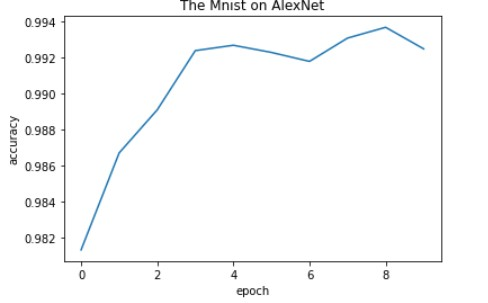
\includegraphics[width=.7\textwidth]{AlexNet1.jpg}
	\caption{LeNet10\_epoch\_acc}
	\label{fig:circuitm1}
\end{figure} \par
\noindent \textbf{AlexNet\_10epoch}\par
\begin{figure}[!h]
	\centering
	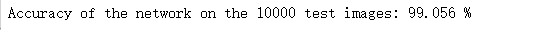
\includegraphics[width=1\textwidth]{结果.jpg}
	\caption{AlexNet\_sqr\_acc}
	\label{fig:circuitm1}
\end{figure} \par
\subsection{GoogLeNet}
inception(也称 GoogLeNet)是 2014 年 Christian Szegedy 提出的一种全新的深度学习结构,在这之前的 AlexNet、VGG 等结构都是通过增大网络的深度(层数)来获得更好的训练效果,但层数的增加会带来很多负作用,比如 overfit、梯度消失、梯度爆炸等。inception 的提出则从另一种角度来提升训练结果:能更高效的利用计算资源,在相同的计算量下能提取到更多的特征,从而提升训练结果。

一般来说,提升网络性能最直接的办法就是增加网络深度和宽度,但一味地增加,会带来诸多问题:
	\begin{enumerate}
	\item [1、] 参数太多,如果训练数据集有限,很容易产生过拟合;
	\item [2、]  网络越大、参数越多,计算复杂度越大,难以应用;
	\item[3、]网络越深,容易出现梯度弥散问题(梯度越往后穿越容易消失),难以优化模型。我们希望在增加网络深度和宽度的同时减少参数,为了减少参数,自然就想到将全连接变成稀疏连接。但是在实现上,全连接变成稀疏连接后实际计算量并不会有质的提升,因为大部分硬件是针对密集矩阵计算优化的,稀疏矩阵虽然数据量少,但是计算所消耗的时间却很难减少。
\end{enumerate}
\subsubsection{inception}
Inception 结构的主要思路是怎样用密集成分来近似最优的局部稀疏结构。\\
\begin{figure}[!h]
	\centering
	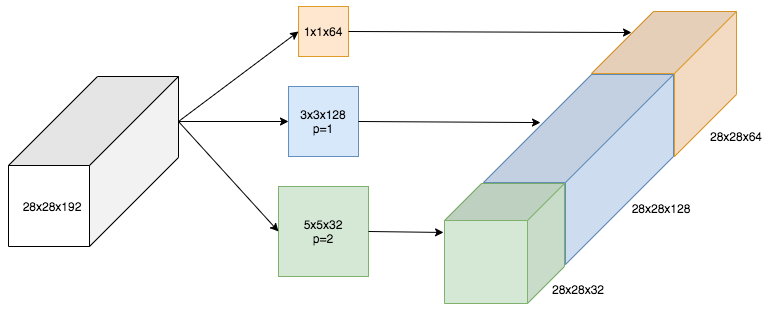
\includegraphics[width=1\textwidth]{goognet.png}
	\caption{Inception块}
	\label{fig:circuitm1}
\end{figure} \par
Naive Inception 单元的详细工作过程,假设在上图中 Naive Inception 单元的前一层输入的数据是一个 32×32×256 的特征图,该特征图先被复制成 4 份并分别被传至接下来的 4 个部分。我们假设这 4 个部分对应的滑动窗口的步长均为 1,其中,1×1 卷积层的 $Padding$ 为 0,滑动窗口维度为 1×1×256,要求输出的特征图深度为 128;3×3 卷积层的 $Padding$ 为 1,滑动窗口维度为 3×3×256,要求输出的特征图深度为 192;5×5 卷积层的 $Padding$为 2,滑动窗口维度为 5×5×256,要求输出的特征图深度为 96;3×3 最大池化层的$Padding$为 1,滑动窗口维度为 3×3×256。这里对每个卷积层要求输出的特征图深度没有特殊意义,仅仅举例用,之后通过计算,分别得到这 4 部分输出的特征图为 32×32×128、32×32×192、32×32×96 和 32×32×256,最后在合并层进行合并,得到 32×32×672 的特征图,合并的方法是将各个部分输出的特征图相加,最后这个 Naive Inception 单元输出的特征图维度是 32×32×672,总的参数量就是 1*1*256*128+3*3*256*192+5*5*256*96=1089536。 
但是 Naive Inception 有两个非常严重的问题:首先,所有卷积层直接和前一层输入的数据对接,所以卷积层中的计算量会很大;其次,在这个单元中使用的最大池化层保留了输入数据的特征图的深度,所以在最后进行合并时,总的输出的特征图的深度只会增加,这样增加了该单元之后的网络结构的计算量。于是人们就要想办法减少参数量来减少计算量,在受到了模型 “Network in Network”的启发,开发出了在 GoogleNet 模型中使用的 Inception 单元(Inception V1),这种方法可以看做是一个额外的 1*1 卷积层再加上一个 ReLU 层。如下所示: 
\begin{figure}[!h]
	\centering
	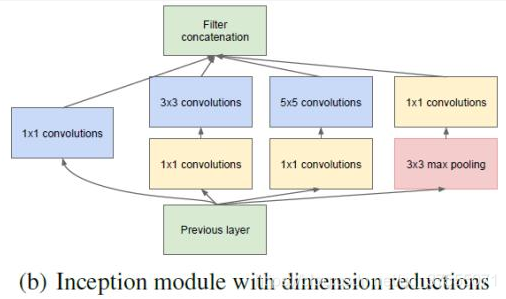
\includegraphics[width=1\textwidth]{inception.png}
	\caption{Inception v1}
	\label{fig:circuitm1}
\end{figure} \par
\subsubsection{Inception块的解释}
    inception 模块的基本机构上图,整个 inception 结构就是由多个这样的 inception 模块串联起来的。inception 结构的主要贡献有两个:一是使用 1x1 的卷积来进行升降维(利用 NiN 的手段);二是在多个尺寸上同时进行卷积再聚合。
\subsubsection{实验结果}
我用GoogLeNet建模失败了,原因不知。它不像AlexNet那样如果出错会出现一个较大的误差,GoogLeNet是一个epoch的均误差,即每个epoch误差都很大,已知道不存在opt的问题。具体原因还未找到,模型的建立可以查我的jupyter实验报告。
\subsection{ResNet}
由于模型建模与googLeNet的相似性,我便未考虑去直接建模。而是尝试用fastai框架去建模,fastai是继承pytorch的一个框架,吸引我使用它的原因是。一方面,我正在读他们的书知道他们数据增强部分做的很好;另一方面建模的流程非常简单,并且采取迁移学习的策略很容易能够达到预期的结果。
\subsubsection{基于fastai的代码框架}
 \begin{lstlisting}[language=python]
 import fastbook
 fastbook.setup_book()
 from fastai.vision.all import *
 from fastbook import *
 matplotlib.rc('image', cmap='Greys')
 path = untar_data(URLs.MNIST)#下载手写数据集
 path.ls()#获取数据集的地址
 # 使用路径创建一个图像数据转换器对象
 dls = ImageDataLoaders.from_folder(path, train='training', 
 valid='testing')# 创建 Dataloader
 learn = cnn_learner(dls, resnet18, pretrained=False,
 loss_func=LabelSmoothingCrossEntropy(),  #标签平滑或者换resnet18
 metrics=accuracy)
 learn.fit_one_cycle(1, 0.1)# 一个epoch,学习率0.1
 # 使用迁移学习训练
 learn.unfreeze()
 learn.lr_find()
 learn.fit_one_cycle(3, slice(1e-6, 1e-4))
	
\end{lstlisting}

\subsubsection{ResNet18及ResNet34对比}
\newpage
\begin{center}
	\textbf{Table 1}~~ ResNet18\\
	\setlength{\tabcolsep}{4mm}{
		\begin{tabular}{ccccc} \toprule
			$epoch$	&$train\_loss$&	$valid\_loss$&$	accuracy$&	$time$\\  
			\hline
		 0	&0.561522&	0.526307&	0.991500&	12:55\\
		 1	&0.559923&	0.525104&	0.990900&	10:18\\
		 2	&0.548604&	0.524869&	0.991600&	10:19\\
		 3	&0.549611&	0.524795&	0.991000&	10:22\\
			\bottomrule
	\end{tabular}}
\end{center}

\begin{center}
	\textbf{Table 2}~~ ResNet34\\
	\setlength{\tabcolsep}{4mm}{
		\begin{tabular}{ccccc} \toprule
			$epoch$	&$train\_loss$&	$valid\_loss$&$	accuracy$&	$time$\\  
			\hline
		0	&0.583426&	0.594473&	0.986200&	22:21\\
		1	&0.578651&	0.543047&	0.987100&	16:14\\
		2	&0.581934&	2.380104&	0.983400&	16:49\\
			\bottomrule
	\end{tabular}}
\end{center}
我们可以看到的是当Mnist选择ResNet18的时候acc反而比ResNet34的效果好,也表明了模型并不是越深越好的事实。通过fastai自带包可以画出学习率图如下:
\begin{figure}[htbp]
	\centering
	\begin{minipage}[t]{0.48\textwidth}
		\centering
		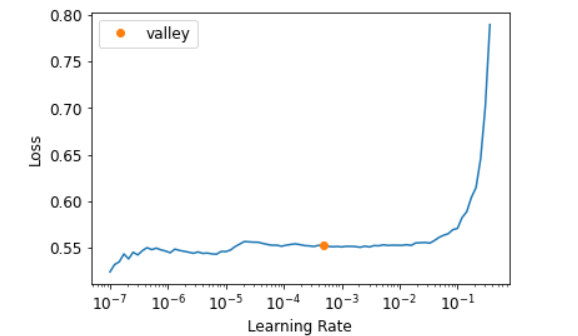
\includegraphics[width=7cm]{19.png}
		\caption{ResNet18 learning-loss}
	\end{minipage}
	\begin{minipage}[t]{0.48\textwidth}
		\centering
		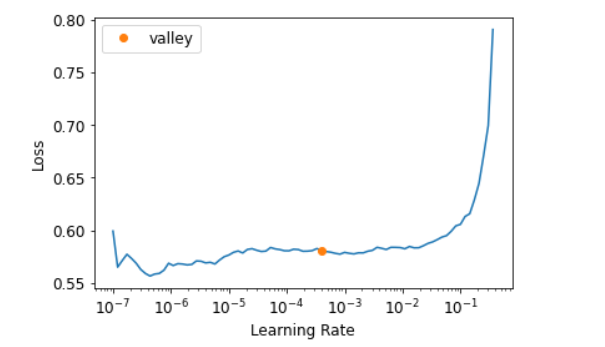
\includegraphics[width=7cm]{20.png}
		\caption{ResNet34 learning-loss}
	\end{minipage}
\end{figure}
 

\section{实验结果分析}
 \subsection{总结}
 Mnist手写数据集本身不是一个复杂的数据集,而且它是单通道的图片,因而建模起来并不复杂。如果数据增强做得好点的话,train部分是可以训练到100\%。但是过多的epoch也可能会导致模型过拟合,从而在test上面acc下降,例如ResNet18和ResNet34,ResNet18的4个epoch平均的acc为99.1\%,而ResNet34却只有98\%。可能就是train过拟合了。在5个网络里,其中训练效果最好的是AlexNet,它的模型效果达到99.26\%。可能也是因为并不复杂的原因。考察5个网络,发现均能超过97\%,可见效果还不错。
 \subsection{改进模型}
 可以进一步做数据增强,fastai中提供了mixup混合形式,这样使得图片直接更加独立。对于googLeNet可以将5x5的卷积核换成3x3的,并且使用1x1降维。不要Resize它的尺寸,直接建模。因为Resize可能会损失图像的一些特征。
 
  

 
\addcontentsline{toc}{section}{参考文献}%将“参考文献加入目录中”
	\begin{thebibliography}{3} 
	\bibitem{ref1}Yu H, Yang L T, Zhang Q, et al. Convolutional neural networks for medical image analysis: state-of-the-art, comparisons, improvement and perspectives[J]. Neurocomputing, 2021, 444: 92-110.
 
	\bibitem{ref2}机器学习及其应用[M]. 清华大学出版社有限公司, 2006. 
	\bibitem{ref3}Targ S, Almeida D, Lyman K. Resnet in resnet: Generalizing residual architectures[J]. arXiv preprint arXiv:1603.08029, 2016.
	 
	
\end{thebibliography}

\newpage

\appendix

\section*{附录A:网络LeNet}
\textbf{\textcolor[rgb]{0.98,0.00,0.00}{ }}
\lstinputlisting[language=Python]{code/Mnist_LeNet.py}

\end{document}